\documentclass[border=10pt]{standalone}
\usepackage{tikz}\usepackage{amsmath}\usetikzlibrary{calc,arrows.meta}
\begin{document}
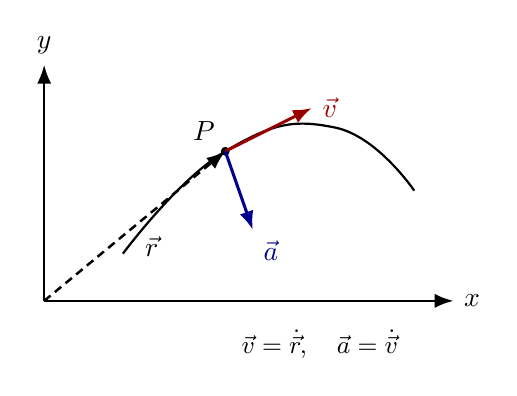
\begin{tikzpicture}[line width=0.9pt,>={Latex[length=2.4mm]}]
  \coordinate (O) at (0,0);
  \draw[->] (O)--(5.2,0) node[right]{$x$};
  \draw[->] (O)--(0,3.0) node[above]{$y$};
  \draw[thick] plot[smooth,tension=0.8] coordinates {(1.0,0.6)(2.3,1.9)(3.7,2.2)(4.7,1.4)};
  \coordinate (P) at (2.3,1.9);
  \fill (P) circle(1.6pt) node[above left]{$P$};
  \draw[->,densely dashed] (O)--(P) node[midway,below right]{$\vec r$};
  \draw[->,red!60!black,line width=1.1pt] (P)--($(P)+(1.1,0.55)$) node[right]{$\vec v$};
  \draw[->,blue!55!black,line width=1.1pt] (P)--($(P)+(0.35,-1.0)$) node[below right]{$\vec a$};
  \node at (3.5,-0.55){\small $\vec v=\dot{\vec r},\quad \vec a=\dot{\vec v}$};
\end{tikzpicture}
\end{document}
